\section{Side by Side comparison}
\label{sec:sidebyside}


In this section we are going to analyse and compare the response generated with the Ngspice simulation and with the Octave tool (Theoretical analysis). 

\begin{figure}[H]
  \centering
  \begin{minipage}[b]{0.45\textwidth}
    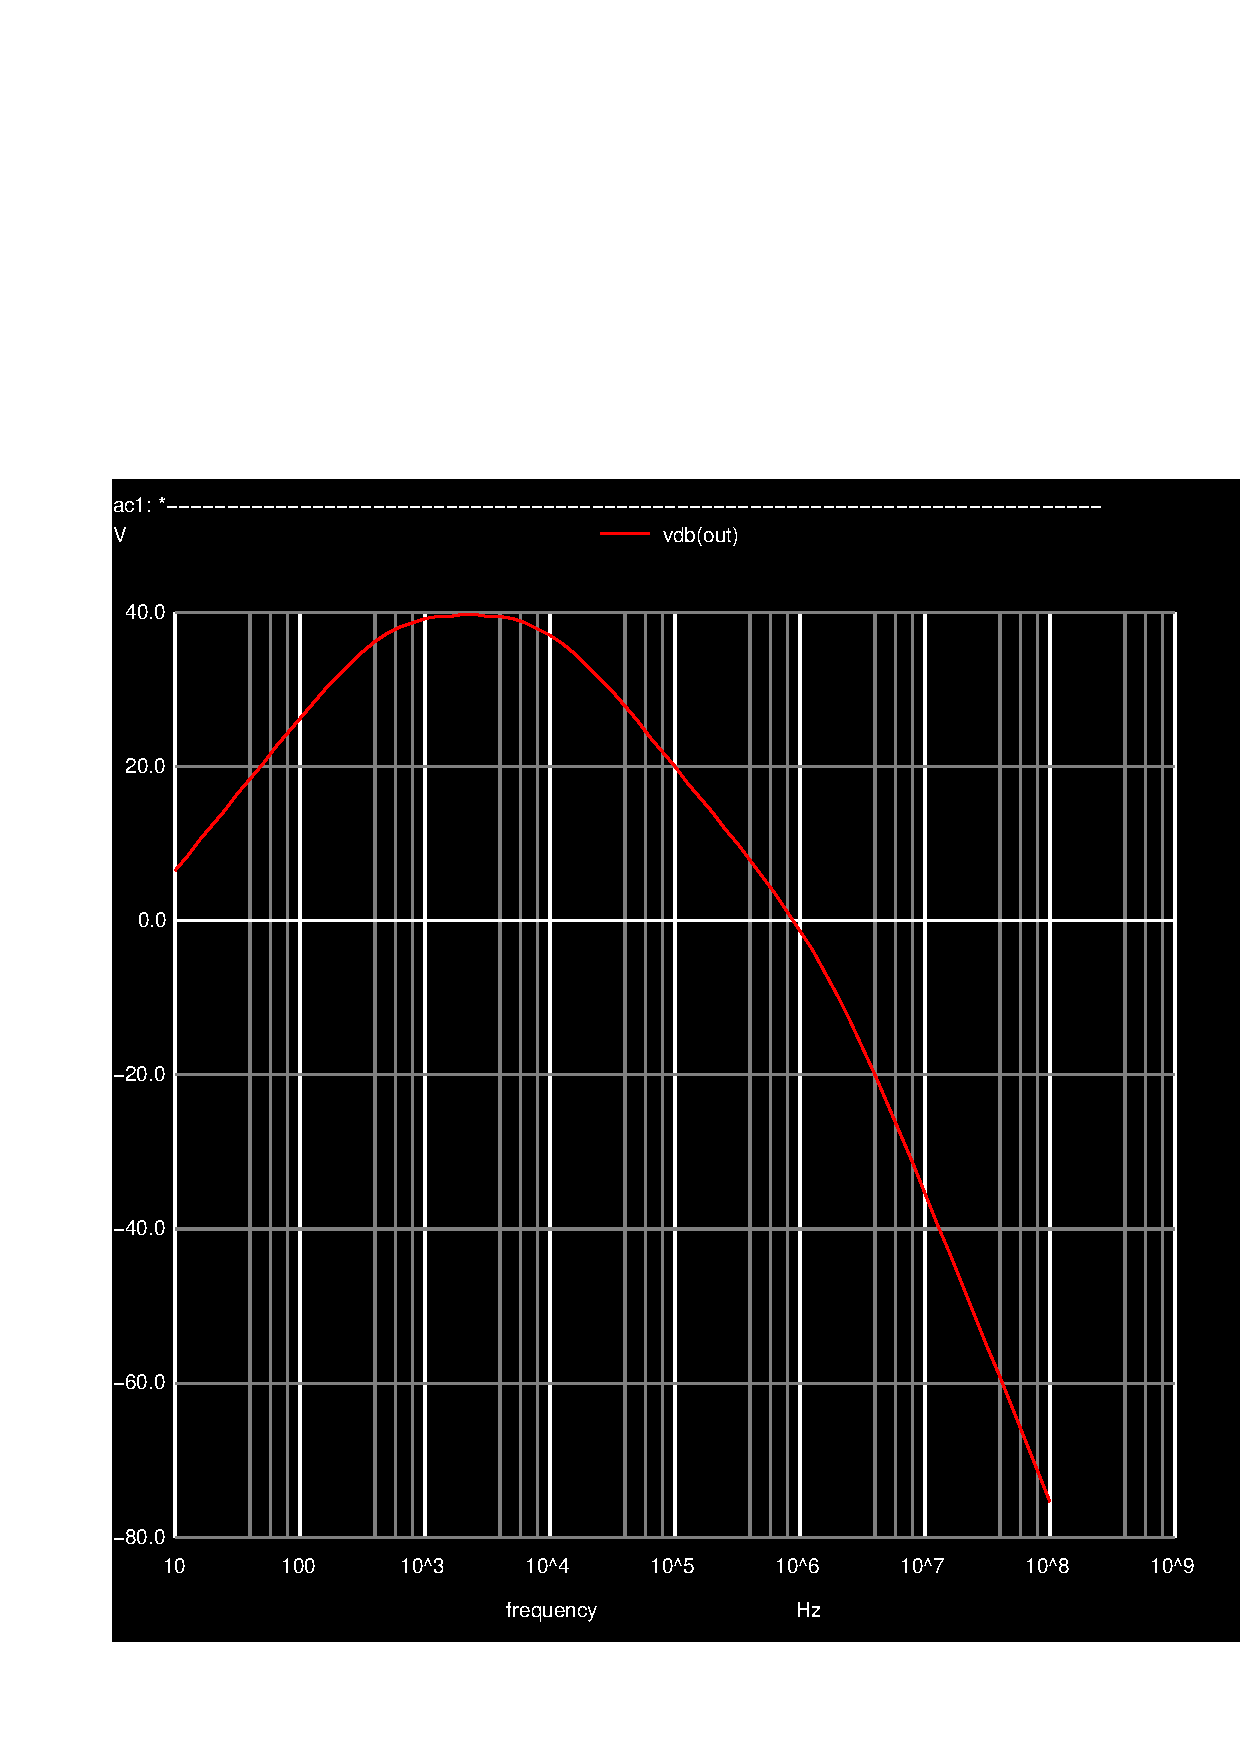
\includegraphics[width=1\textwidth]{vo1db.pdf}
    \caption{Simulation response}
    \label{fig:label_02}
  \end{minipage}
  \hfill
  \begin{minipage}[b]{0.52\textwidth}
    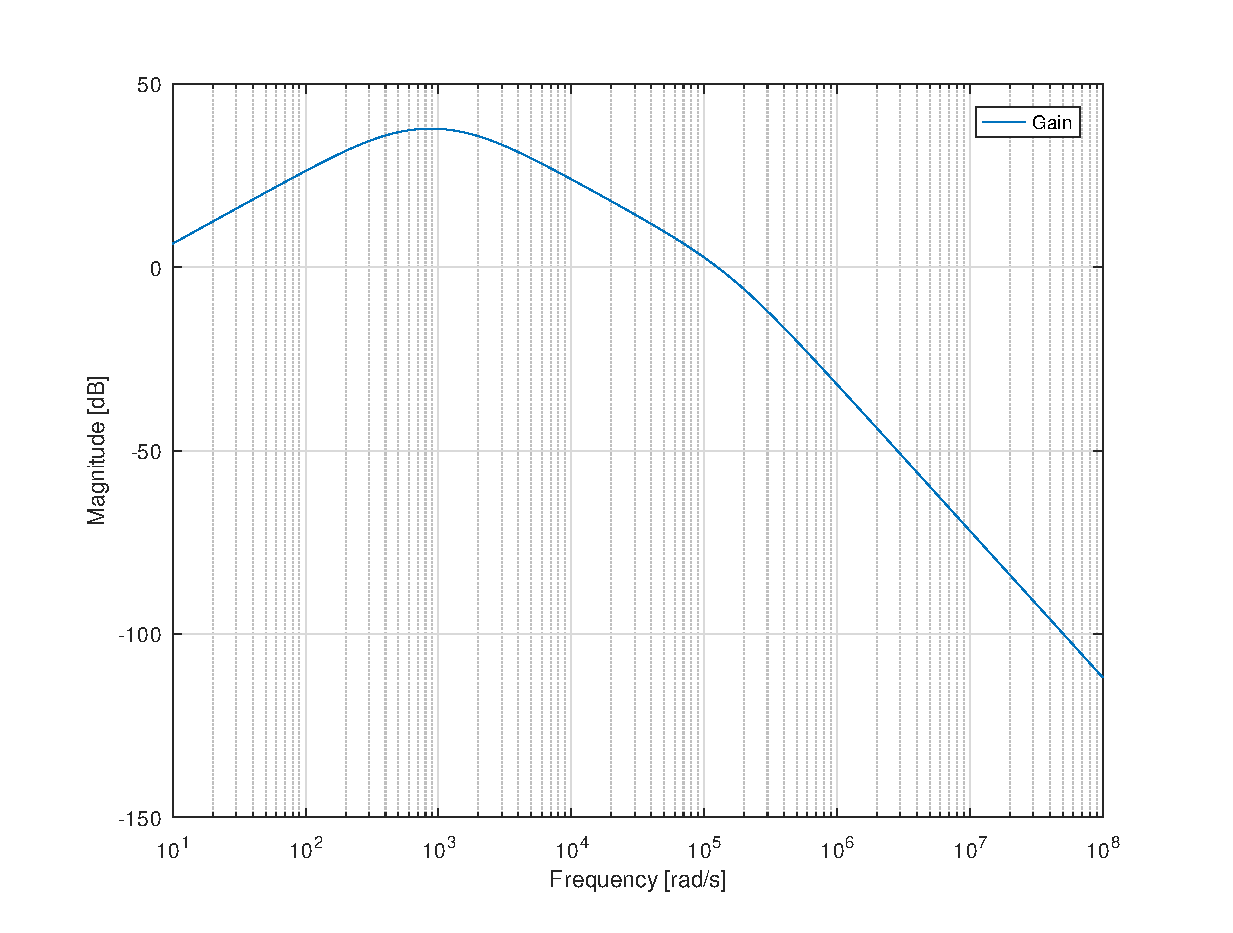
\includegraphics[width=1\textwidth]{b3.eps}
    \caption{Theoretical response}
    \label{fig:label_03}
  \end{minipage}
\end{figure}

As we can see, the simulation and theoretical analysis responses are very similars.
The fact that the visualization is being done in logarithmic scales makes small discrepancies completely impossible to visualize. 

